\chude{Ứng dụng diện tích hình phẳng và thể tích khối tròn xoay trong bài toán thực tiễn}

\begin{dang}{Ứng dụng diện tích hình phẳng trong bài toán thực tiễn}
\end{dang}

\Opensolutionfile{ans}[ans/ans-2-C4B3CD3_1-4-lc]
\TN

%Câu 1
\begin{ex}%[2D4V3-2]
	Trường Nguyễn Văn Trỗi muốn làm một cái cửa nhà hình parabol có chiều cao từ mặt đất đến đỉnh là $2{,}25$\,mét, chiều rộng tiếp giáp với mặt đất là $3$\,mét. Giá thuê mỗi mét vuông là $1\,500\,000$\,đồng. Vậy số tiền nhà trường phải trả là
	\choice
	{$33\,750\,000$\,đồng}
	{$3\,750\,000$\,đồng}
	{$12\,750\,000$\,đồng}
	{\True $6\,750\,000$\,đồng}
	\loigiai{
		\immini{Gọi phương trình parabol
			\[(P)\colon y=ax^2+bx+c.\]
		Do tính đối xứng của parabol nên ta có thể chọn hệ trục tọa độ $Oxy$ sao cho $(P)$ có đỉnh $I\in Oy$ (như hình vẽ).\\
		Ta có hệ phương trình\\ $\heva{&\dfrac{9}{4}=c,\Big(I\in(P)\Big)\\&\dfrac{9}{4}a-\dfrac{3}{2}b+c=0\Big(A\in(P)\Big)\\&\dfrac{9}{4}a+\dfrac{3}{2}b+c=0\Big(B\in(P)\Big)} \Leftrightarrow \heva{&c=\dfrac{9}{4}\\&a=-1\\& b=0.}$\\
		Vậy $(P)\colon y=-x^2+\dfrac{9}{4}$.
		}{
				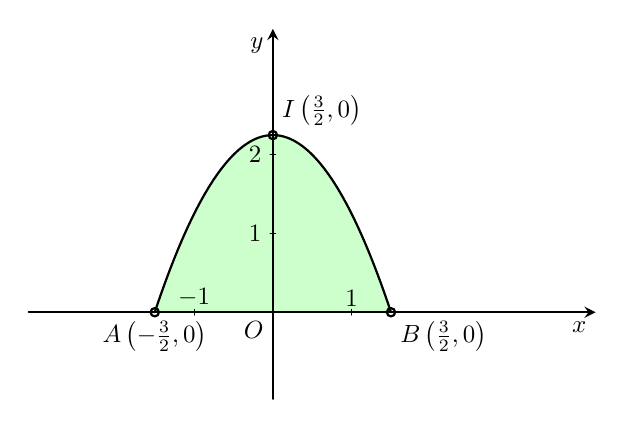
\begin{tikzpicture}[line join=round, line cap=round,>=stealth,thick]
					\tikzset{every node/.style={scale=0.9}}
					\begin{scope}
						\clip (-3,-1) rectangle (3,3.5);
						\draw[fill=green!20](-1.5,0)--plot[samples=200,domain=-1.5:1.5,smooth,variable=\x] (\x,{-1*(\x)^2+9/4})--(1.5,0);
						\draw (-1.5,0) circle (1.5pt) node[below]{$A\left(-\frac{3}{2},0\right)$};
						\draw (1.5,0) circle (1.5pt) node[below right]{$B\left(\frac{3}{2},0\right)$};
						\draw (0,2.25) circle (1.5pt) node[above right]{$I\left(\frac{3}{2},0\right)$};
					\end{scope}
					\draw[->] (-3.1,0)--(4.1,0) node[below left] {$x$};
					\draw[->] (0,-1.1)--(0,3.6) node[below left] {$y$};
					\draw (0,0) node [below left] {$O$};
					\foreach \x/\nx in {-1/-1,1/1}
					\draw[thin] (\x,1pt)--(\x,-1pt) node [above] {$\nx$};
					\foreach \y/\ny in {1/1,2/2}
					\draw[thin] (1pt,\y)--(-1pt,\y) node [left] {$\ny$};
				\end{tikzpicture}
		}
		\noindent
		Dựa vào đồ thị, diện tích của parabol là
		\[S=\displaystyle\int\limits_{-\tfrac{3}{2}}^{\tfrac{3}{2}}{\left(-x^2+\dfrac{9}{4}\right)\mathrm{\,d}x}=2\displaystyle\int\limits_0^{\tfrac{3}{2}}{\left(-x^2+\dfrac{9}{4}\right)\mathrm{\,d}x}=2\left(\dfrac{-x^3}{3}+\dfrac{9}{4}x\right)\Bigg|_0^{\tfrac{9}{4}}=\dfrac{9}{2}\,\mathrm{(m^2)}.\]
		Số tiền phải trả là $\dfrac{9}{2}\cdot 1\,500\,000=6\,750\,000$\,(đồng).
		}
\end{ex}

%Câu 2
\begin{ex}%[2D4V3-2]
	\immini{Chị Minh Hiền muốn làm một cái cổng hình Parabol như hình vẽ bên. Chiều cao $GH=4$\,m, chiều rộng $AB=4$\,m, $AC=BD=0{,}9$\,m. Chị Minh Hiền làm hai cánh cổng khi đóng lại là hình chữ nhật $CDEF$ tô đậm có giá là $1\,200\,000$\,đồng/$\mathrm{m^2}$, còn các phần để trắng làm xiên hoa có giá là $900\,000$\,đồng/$\mathrm{m^2}$. Hỏi tổng số tiền để làm hai phần nói trên gần nhất với số tiền nào dưới đây?
	\choice
	{\True $11\,445\,000$\,đồng}
	{$4\,077\,000$\,đồng}
	{$7\,368\,000$\,đồng}
	{$11\,370\,000$\,đồng}
	}{
		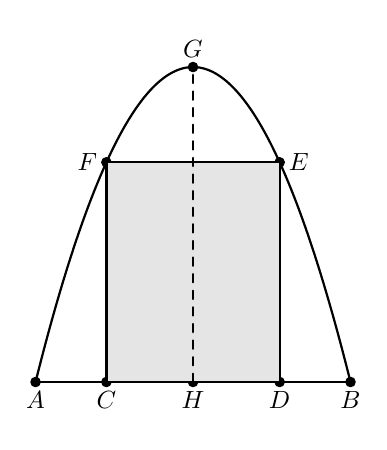
\begin{tikzpicture}[line join=round, line cap=round,>=stealth,thick]
			\tikzset{every node/.style={scale=0.9}}
			\begin{scope}
				\clip (-0.1,-0.5) rectangle (4.1,4.5);
				\draw(0,0)--plot[samples=200,domain=0:4,smooth,variable=\x] (\x,{-1*(\x)^2+4*(\x)})--(4,0);
				\draw[fill=black](0,0) circle (1.5pt) node[below]{$A$} (4,0) circle (1.5pt) node[below]{$B$} (2,4) circle (1.5pt) node[above]{$G$} (0.9,2.79) circle (1.5pt) node[left]{$F$} (3.1,2.79) circle (1.5pt) node[right]{$E$} (3.1,0) circle (1.5pt) node[below]{$D$} (0.9,0) circle (1.5pt) node[below]{$C$} (2,0) circle (1.5pt) node[below]{$H$};
				\draw[fill=gray!20](0.9,0)--(0.9,2.79)--(3.1,2.79)--(3.1,0) (0,0)--(4,0);
				\draw[dashed](2,0)--(2,4);
			\end{scope}
		\end{tikzpicture}
	}
	\loigiai{
			\immini{Gắn hệ trục tọa độ Oxy sao cho $AB$ trùng $Ox$, $A$ trùng $O$ khi đó parabol có đỉnh $G(2;4)$ và đi qua gốc tọa độ.\\
			Giả sử phương trình của parabol có dạng $y=ax^2+bx+c$, $(a\ne 0)$.\\
			Vì parabol có đỉnh là $G(2;4)$ và đi qua điểm $O(0;0)$ nên ta có \[\heva{&c=0\\&-\dfrac{b}{2a}=2\\&a\cdot 2^2+b\cdot 2+c=4}\Leftrightarrow\heva{&a=-1\\&b=4\\&c=0.}\]
			}{
				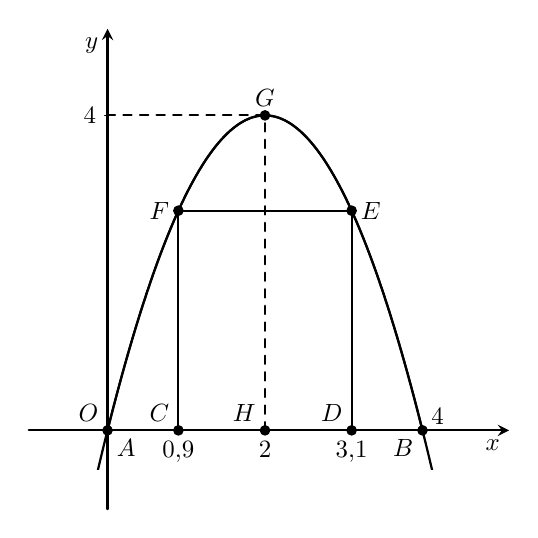
\begin{tikzpicture}[line join=round, line cap=round,>=stealth,thick]
				\tikzset{every node/.style={scale=0.9}}
				\begin{scope}
				\clip (-0.5,-0.5) rectangle (4.5,4.5);
				\draw(0,0)--plot[samples=200,domain=0:4,smooth,variable=\x] (\x,{-1*(\x)^2+4*(\x)})--(4,0);
				\draw plot[samples=200,domain=-0.5:4.5,smooth,variable=\x] (\x,{-1*(\x)^2+4*(\x)});
				\draw[fill=black](0,0) circle (1.5pt) node[below right]{$A$} (4,0) circle (1.5pt) node[below left]{$B$} (2,4) circle (1.5pt) node[above]{$G$} (0.9,2.79) circle (1.5pt) node[left]{$F$} (3.1,2.79) circle (1.5pt) node[right]{$E$} (3.1,0) circle (1.5pt) node[above left]{$D$} (0.9,0) circle (1.5pt) node[above left]{$C$} (2,0) circle (1.5pt) node[above left]{$H$};
				\draw(0.9,0)--(0.9,2.79)--(3.1,2.79)--(3.1,0) (0,0)--(4,0);
				\draw[dashed](2,0)--(2,4)--(0,4);
				\end{scope}
				\draw[->] (-1,0)--(5.1,0) node[below left] {$x$};
				\draw[->] (0,-1)--(0,5.1) node[below left] {$y$};
				\draw (0,0) node [above left] {$O$};
				\foreach \x/\nx in {0.9/0{,}9,2/2,3.1/3{,}1}
				\draw[thin] (\x,1pt)--(\x,-1pt) node [below] {$\nx$};
				\draw[thin] (4,1pt)--(4,-1pt) node [above right] {$4$};
				\foreach \y/\ny in {4/4}
				\draw[thin] (1pt,\y)--(-1pt,\y) node [left] {$\ny$};
				\end{tikzpicture}				
			}
			\noindent
			Suy ra phương trình parabol là $y=f(x)=-x^2+4x$.\\
			Diện tích của cả cổng là $S=\displaystyle\int\limits_0^4\left(-x^2+4x\right)\mathrm{\,d}x=\left(-\dfrac{x^3}{3}+2x^2\right)\Bigg|_0^4=\dfrac{32}{3}\,\mathrm{\left(m^2\right)}$.\\
			Mặt khác chiều cao $CF=DE=f(0{,}9)=2{,}79$\,(m); $CD=4-2\cdot 0{,}9=2{,}2$\,(m).\\
			Diện tích hai cánh cổng là $S_{CDEF}=CD\cdot CF=6{,}138\,\mathrm{(m^2)}$.\\
			Diện tích phần xiên hoa là $S_{xh}=S-S_{CDEF}=\dfrac{32}{3}-6{,}14=\dfrac{6793}{1500}\,\mathrm{(m^2)}$.\\
			Vậy tổng số tiền để làm cổng là $6{,}138\cdot 1\,200\,000+\dfrac{6793}{1500}\cdot 900\,000=11\,441\,400$\,(đồng).
			}
\end{ex}
	
%Câu 3
\begin{ex}%[2D4V3-2]
		\immini{Một cổng chào có dạng hình Parabol chiều cao $18$\,m, chiều rộng chân đế $12$\,m. Người ta căng hai sợi dây trang trí $AB$, $CD$ nằm ngang đồng thời chia hình giới hạn bởi Parabol và mặt đất thành ba phần có diện tích bằng nhau (xem hình vẽ bên). Tỉ số $\dfrac{AB}{CD}$ bằng
		\choice
		{$\dfrac{1}{\sqrt{2}}$}
		{$\dfrac{4}{5}$}
		{\True $\dfrac{1}{\sqrt[3]{2}}$}
		{$\dfrac{3}{1+2\sqrt{2}}$}
		}{
		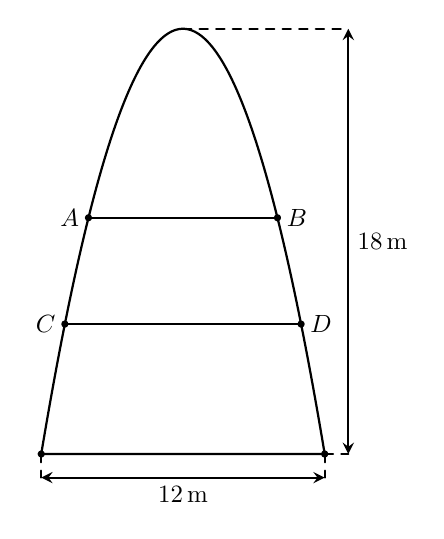
\begin{tikzpicture}[line join=round, line cap=round,>=stealth,thick,scale=0.6]
			\tikzset{every node/.style={scale=0.9}}
			\begin{scope}
				\draw(-3,-9)--plot[samples=200,domain=-3:3,smooth,variable=\x] (\x,{-1*(\x)^2})--(3,-9)--cycle;
				\draw[dashed](0,0)--(3.5,0) (3,-9)--(3.5,-9) (-3,-9)--(-3,-9.5) (3,-9)--(3,-9.5);
				\draw[<->](3.5,0)--(3.5,-9) node[pos=0.5, right]{$18$\,m}; \draw[<->](-3,-9.5)--(3,-9.5) node[pos=0.5, below]{$12$\,m};
				\draw[fill=black](-2,-4) circle (1.5pt) node[left]{$A$} (2,-4) circle (1.5pt) node[right]{$B$} (-2.5,-6.25) circle (1.5pt) node[left]{$C$} (2.5,-6.25) circle (1.5pt) node[right]{$D$} (-3,-9) circle (1.5pt) (3,-9) circle (1.5pt);
				\draw (-2,-4)--(2,-4) (-2.5,-6.25)--(2.5,-6.25);
			\end{scope}
		\end{tikzpicture}
		}
		\loigiai{
			\immini{Chọn hệ trục tọa độ $Oxy$ như hình vẽ.
			Phương trình Parabol $(P)$ có dạng $y=ax^2$.\\
			$(P)$ đi qua điểm có tọa độ $(-6;-18)$.\\
			Suy ra $-18=a\cdot (-6)^2\Leftrightarrow a=-\dfrac{1}{2}.\\
			\Rightarrow(P)\colon y=-\dfrac{1}{2}x^2$.\\
			Từ hình vẽ ta có $\dfrac{AB}{CD}=\dfrac{x_1}{x_2}$.\\
			Diện tích hình phẳng giới bạn bởi Parabol và đường thẳng $AB\colon y=-\dfrac{1}{2}x_1^2$ là
			\allowdisplaybreaks
			\begin{eqnarray*}
				S_1&=&2\displaystyle\int\limits_0^{x_1}{\left[-\dfrac{1}{2}{x^2}-\left(-\dfrac{1}{2}x_1^2\right)\right]\mathrm{\,d}x}\\
				&=&2\left(-\dfrac{1}{2}\cdot \dfrac{x^3}{3}+\dfrac{1}{2}x_1^2x\right)\Bigg|_0^{x_1}=\dfrac{2}{3}x_1^3.
			\end{eqnarray*}
			}{
				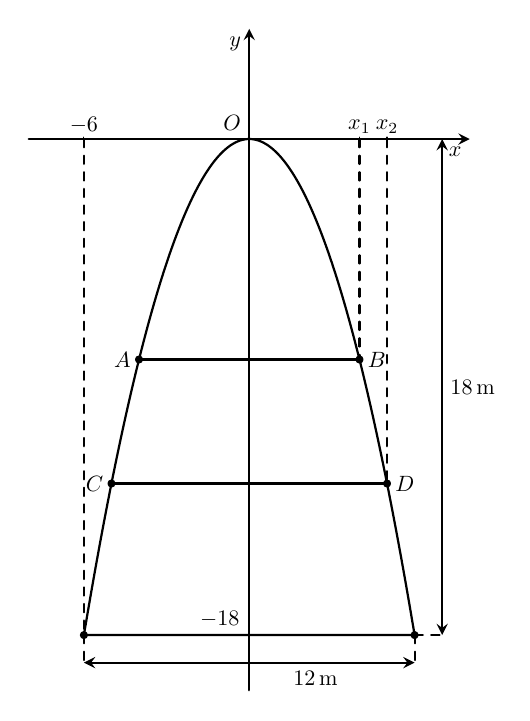
\begin{tikzpicture}[line join=round, line cap=round,>=stealth,thick,scale=0.7]
					\tikzset{every node/.style={scale=0.8}}
					\begin{scope}
						\draw(-3,-9)--plot[samples=200,domain=-3:3,smooth,variable=\x] (\x,{-1*(\x)^2})--(3,-9)--cycle;
						\draw[dashed] (3,-9)--(3.5,-9) (-3,-9)--(-3,-9.5) (3,-9)--(3,-9.5);
						\draw[<->](3.5,0)--(3.5,-9) node[pos=0.5, right]{$18$\,m}; \draw[<->](-3,-9.5)--(3,-9.5) node[pos=0.7, below]{$12$\,m};
						\draw[fill=black](-2,-4) circle (1.5pt) node[left]{$A$} (2,-4) circle (1.5pt) node[right]{$B$} (-2.5,-6.25) circle (1.5pt) node[left]{$C$} (2.5,-6.25) circle (1.5pt) node[right]{$D$} (-3,-9) circle (1.5pt) (3,-9) circle (1.5pt);
						\draw (-2,-4)--(2,-4) (-2.5,-6.25)--(2.5,-6.25);
					\end{scope}
					\draw[->] (-4,0)--(4,0) node[below left] {$x$};
					\draw[->] (0,-10)--(0,2.0) node[below left] {$y$};
					\draw (0,0) node [above left] {$O$};
					\foreach \x/\nx in {-3/-6,2/x_1,2.5/x_2}
					\draw[thin] (\x,1pt)--(\x,-1pt) node [above] {$\nx$};
					\draw[thin] (1pt,-9)--(-1pt,-9) node [above left] {$-18$};
					\draw[dashed](-3,0)--(-3,-9) (2,0)--(2,-4) (2.5,0)--(2.5,-6.25);
				\end{tikzpicture}
			}
			\noindent
			Diện tích hình phẳng giới hạn bởi Parabol và đường thẳng $CD\colon y=-\dfrac{1}{2}x_2^2$ là
			\[S_2=2\displaystyle\int\limits_0^{x_2}{\left[-\dfrac{1}{2}{x^2}-\left(-\dfrac{1}{2}x_2^2\right)\right]\mathrm{\,d}x}=2\left(-\dfrac{1}{2}\cdot \dfrac{x^3}{3}+\dfrac{1}{2}x_2^2x\right)\Bigg|_0^{x_2}=\dfrac{2}{3}x_2^3.\]
			Từ giả thiết suy ra $S_2=2S_1\Leftrightarrow x_2^3=2x_1^3\Leftrightarrow\dfrac{x_1}{x_2}=\dfrac{1}{\sqrt[3]{2}}$.\\
			Vậy $\dfrac{AB}{CD}=\dfrac{x_1}{x_2}=\dfrac{1}{\sqrt[3]{2}}$.
			}
\end{ex}
	
%Câu 4
\begin{ex}%[2D4C3-2]
		\immini{Một họa tiết hình cánh bướm như hình vẽ bên. Phần tô đậm được đính đá với giá thành $500\,000$/$\,\mathrm{m^2}$. Phần còn lại được tô màu với giá thành $250\,000$/$\,\mathrm{m^2}$. Cho $AB=4$\,dm; $BC=8$\,dm. Hỏi để trang trí $1\,000$ họa tiết như vậy cần số tiền gần nhất với số nào sau đây.
		\choice
		{$105\,660\,667$}
		{\True $106\,666\,667$}
		{$ 107\,665\,667$}
		{$ 108\,665\,667$}
		}{
			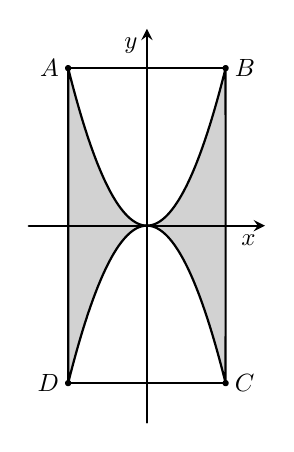
\begin{tikzpicture}[line join=round, line cap=round,>=stealth,thick,scale=0.5]
				\tikzset{every node/.style={scale=0.9}}
				\begin{scope}
					\draw[fill=gray!35](-2,0)--plot[samples=200,domain=-2:2,smooth,variable=\x] (\x,{(\x)^2})--(2,0);
					\draw[fill=gray!35](-2,0)--plot[samples=200,domain=-2:2,smooth,variable=\x] (\x,{-1*(\x)^2})--(2,0);
					\draw[fill=black](-2,4) circle (1.5pt) node[left]{$A$} (2,4) circle (1.5pt) node[right]{$B$} (2,-4) circle (1.5pt) node[right]{$C$} (-2,-4) circle (1.5pt) node[left]{$D$};
					\draw (-2,4)--(2,4) (2,-4)--(-2,-4);
				\end{scope}
				\draw[->] (-3,0)--(3,0) node[below left] {$x$};
				\draw[->] (0,-5)--(0,5) node[below left] {$y$};
			\end{tikzpicture}
		}
		\loigiai{
			Vì $AB=4$\,dm; $BC=8$\,dm $\Rightarrow A(-2;4)$, $B(2;4)$, $C(2;-4)$, $D(-2;-4)$.\\
			parabol là $y=x^2$ hoặc $y=-x^2$.\\
			Diện tích phần tô đậm là $S_1=4\displaystyle\int\limits_0^2{x^2}\mathrm{\,d}x=\dfrac{32}{3}\mathrm{\,(dm^2)}$.\\
			Diện tích hình chữ nhật là $S=4\cdot 8=32\mathrm{\,(dm^2)}$.\\
			Diện tích phần trắng là $S_2=S-S_1=32-\dfrac{32}{3}=\dfrac{64}{3}\mathrm{\,(dm^2)}$.\\
			Tổng chi phí trang chí là $T=\left(\dfrac{32}{3}\cdot 5\,000+\dfrac{64}{3}\cdot 2\,500\right)\cdot 1\,000\approx 106\,666\,667$.
			}
\end{ex}
	
%Câu 5
\begin{ex}%[2D4C3-2]
		\immini{Một hoa văn trang trí được tạo ra từ một miếng bìa mỏng hình vuông cạnh bằng $10$\,cm bằng cách khoét đi bốn phần bằng nhau có hình dạng parabol như hình bên. Biết $AB=5$\,cm, $OH=4$\,cm. Biết giá trang trí hoa văn $1\mathrm{cm^2}$ là $50\,000$\,đồng, tính số tiền cần bỏ ra để trang trí hoa văn đó.
		\choice
		{$2\,553\,333$\,đồng}
		{\True $2\,333\,333$\,đồng}
		{$2\,780\,333$\,đồng}
		{$2\,123\,333$\,đồng}
		}{
			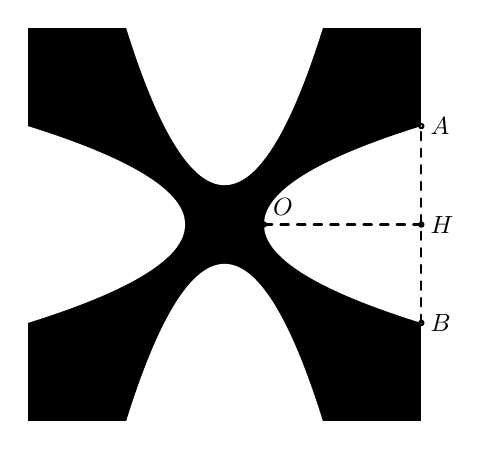
\begin{tikzpicture}[line join=round, line cap=round,>=stealth,thick,scale=0.5]
			\tikzset{every node/.style={scale=0.9}}
				\begin{scope}
					\fill[black] (0,0)--(10,0)--(10,10)--(0,10)--cycle;
					\fill[white](2.5,0)--plot[samples=200,domain=2.5:7.5,smooth,variable=\x] (\x,{-16/25*(\x-2.5)^2+16/5*(\x-2.5)})--(7.5,0);
					\fill[white](2.5,10)--plot[samples=200,domain=2.5:7.5,smooth,variable=\x] (\x,{16/25*(\x-2.5)^2-16/5*(\x-2.5)+10})--(7.5,10);
					\fill[white] plot[samples=200,domain=6:10,smooth,variable=\x] (\x,{sqrt(1.5625*((\x)-6))+5})--(10,5)--plot[samples=200,domain=6:10,smooth,variable=\x] (\x,{-sqrt(1.5625*((\x)-6))+5})--(10,5);
					\fill[white] plot[samples=200,domain=4:0,smooth,variable=\x] (\x,{sqrt(1.5625*(4-(\x)))+5})--(0,5)--plot[samples=200,domain=4:0,smooth,variable=\x] (\x,{-sqrt(1.5625*(4-(\x)))+5})--(0,5);				
				\end{scope}
				\draw[fill=white](6,5) circle (1.5pt) node[above right]{$O$} (10,2.5) circle (1.5pt) node[right]{$B$} (10,7.5) circle (1.5pt) node[right]{$A$} (10,5) circle (1.5pt) node[right]{$H$};
				\draw[dashed] (6,5)--(10,5) (10,2.5)--(10,7.5);
			\end{tikzpicture}
		}
		\loigiai{
		\immini{Đưa parabol vào hệ trục $Oxy$ ta tìm được phương trình là $(P)\colon y=-\dfrac{16}{25}x^2+\dfrac{16}{5}x$.\\
		Diện tích hình phẳng giới hạn bởi $(P)\colon y=-\dfrac{16}{25}x^2+\dfrac{16}{5}x$, trục hoành và các đường thẳng $x=0$, $x=5$ là
		\[S=\displaystyle\int\limits_0^5{\left(-\dfrac{16}{25}x^2+\dfrac{16}{5}x\right)\mathrm{\,d}x}=\dfrac{40}{3}.\]
		}{
			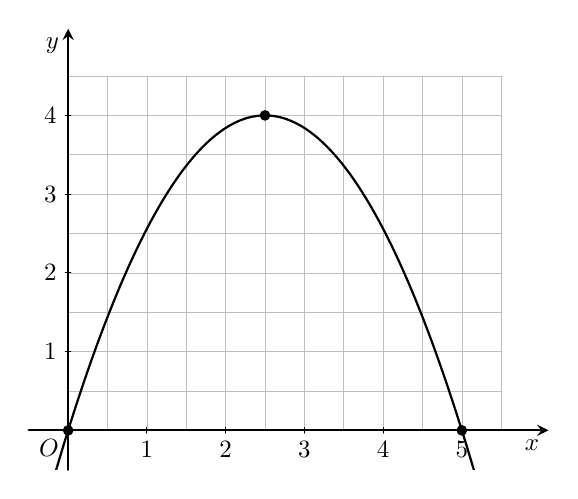
\begin{tikzpicture}[line join=round, line cap=round,>=stealth,thick]
			\tikzset{every node/.style={scale=0.9}}
			\draw[step=0.5, gray!50,very thin] (0,0) grid (5.5,4.5);
			\draw[->] (-0.5,0)--(6.1,0) node[below left] {$x$};
			\draw[->] (0,-0.5)--(0,5.1) node[below left] {$y$};
			\foreach \x/\nx in {1/1,2/2,3/3,4/4,5/5}
			\draw[thin] (\x,1pt)--(\x,-1pt) node [below] {$\nx$};
			\foreach \y/\ny in {1/1,2/2,3/3,4/4}
			\draw[thin] (1pt,\y)--(-1pt,\y) node [left] {$\ny$};
			\draw (0,0) node [below left] {$O$};
			\begin{scope}
				\clip (-0.5,-0.5) rectangle (5.5,5);
				\draw[samples=200,domain=-0.5:5.5,smooth,variable=\x] plot (\x,{-0.64*(\x)^2+3.2*(\x)+0});
			\end{scope}
			\draw[fill=black](0,0) circle (1.5pt) (2.5,4) circle (1.5pt) (5,0) circle (1.5pt);
			\end{tikzpicture}		
		}
		\hspace{-0.8cm}
		Tổng diện tích phần bị khoét đi $S_1=4S=\dfrac{160}{3}\mathrm{\,(cm^2)}$.\\
		Diện tích của hình vuông là $S_{hv}=100\mathrm{\,(cm^2)}$.\\
		diện tích bề mặt hoa văn là $S_2=S_{hv}-S_1=100-\dfrac{160}{3}=\dfrac{140}{3}\mathrm{\,(cm^2)}$.\\
		Vậy số tiền cần bỏ ra để trang trí hoa văn đó là $\dfrac{140}{3}\cdot 50\,000\approx 2\,333\,333$\,(đồng).
	}
\end{ex}

\Closesolutionfile{ans}
\indapan{6}{ans/ans-2-C4B3CD3_1-4-lc}

%\TNTF
%\Opensolutionfile{ans}[ans/ans-2-B1-DS]
%
%\Closesolutionfile{ans}
%\indapan{3}{ans/ans-2-B1-DS}
%
%\Opensolutionfile{ans}[ans/ans-2-B1-KQ]
%\TNSA
%
%\Closesolutionfile{ans}
%\indapan{6}{ans/ans-2-B1-KQ}